\subsection{Datasets} \label{sec:dataset}

\paragraph{DeepFashion2}

\begin{figure} [H]
    \centering
    \captionsetup{justification=centering}
    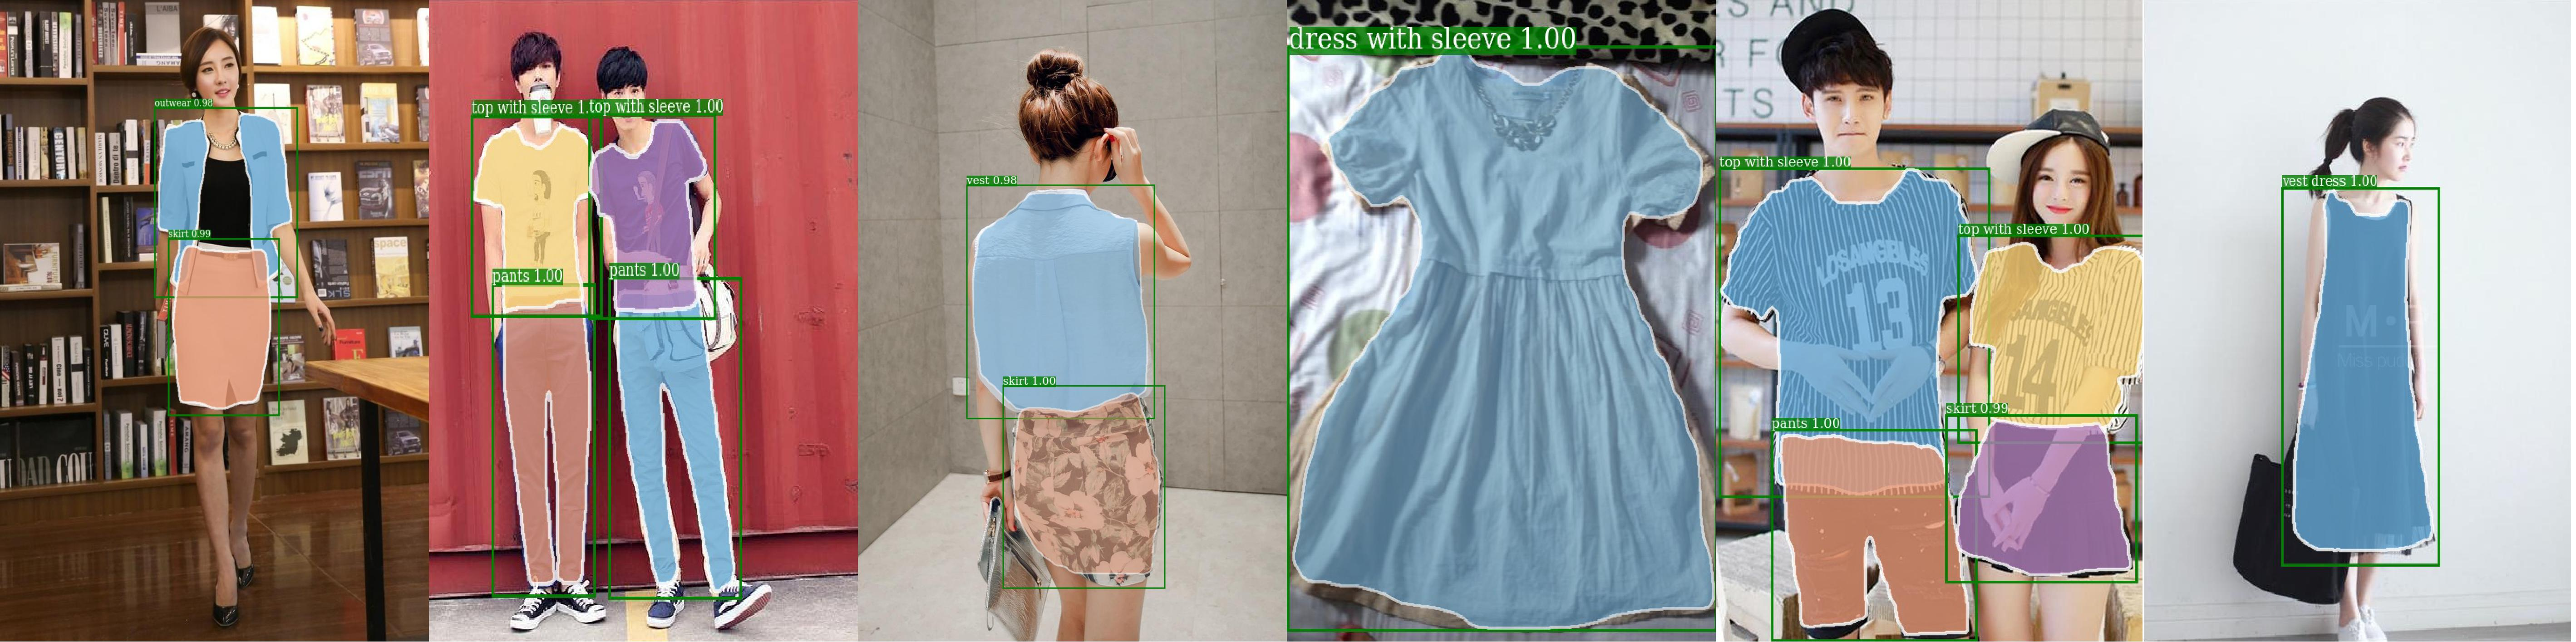
\includegraphics[width=0.9\textwidth]{chapter4/image/deepfashion20.jpg}
    \caption{Polygon annotation examples in DeepFashion2 dataset}
    \label{fig:df}
\end{figure}

DeepFashion is a large-scale clothes dataset with over 800.000 images of 46 clothing categories under different scenarios, namely street snapshot, store. DeepFashion2 is an extension of DeepFashion, proposed to study a broad spectrum of computer vision applications for fashion, including clothes retrieval, clothes recommendation, and virtual try-on. Applied for comprehensive tasks, DeepFashion2 has richer annotations such as style, bounding box, viewpoint, scale, etc. It contains 491.000 images of 13 clothing categories. Here is the identity number and name of the whole thirteen categories: 1 represents short sleeve top, 2 represents long sleeve top, 3 represents short sleeve outwear, 4 represents long sleeve outwear, 5 represents vest, 6 represents sling, 7 represents shorts, 8 represents trousers, 9 represents skirt, 10 represents short sleeve dress, 11 represents long sleeve dress, 12 represents vest dress and 13 represents sling dress. \par 

\begin{figure} [H]
    \centering
    \captionsetup{justification=centering}
    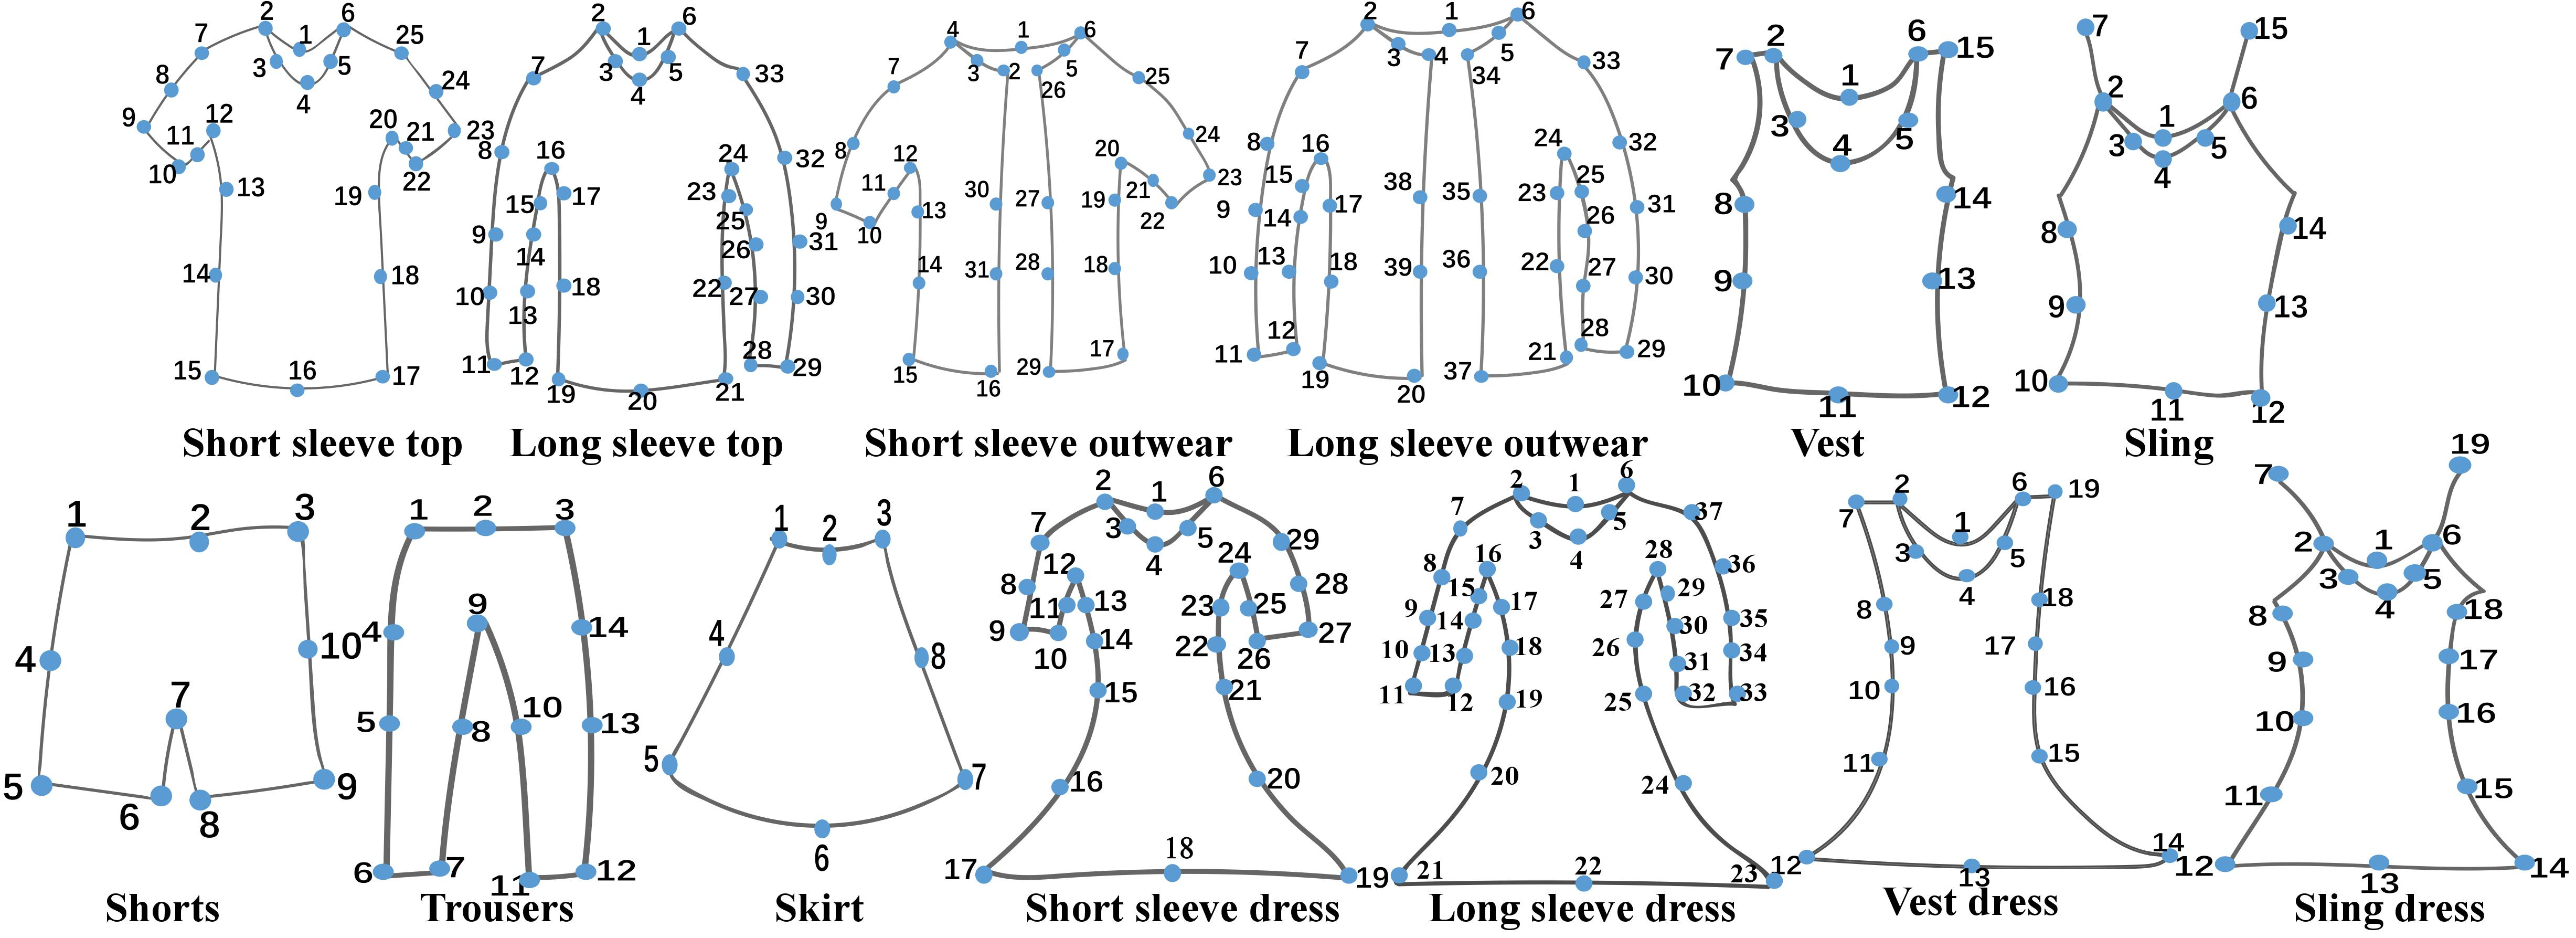
\includegraphics[width=0.9\textwidth]{chapter4/image/deepfahsion2_class.jpg}
    \caption{Thirteen categories of DeepFashion2 dataset}
    \label{fig:dfcate}
\end{figure}

However, I only use the dataset for upper-body clothes (includes the first six categories) recognition. Thus images with categories from 6 to 13 are excluded. After removing lower-body clothes, the dataset remains 137,850 images in the training set. \par


\noindent Differences when compare DeepFashion2 with DeepFashion:
\begin{itemize}
\item DeepFashion2 includes multiple items (pieces of clothing) in an image, while DeepFashion only has a single item per image.
\item DeepFashion is annotated with sparse landmarks per, each piece of cloth only has from 4 to 8 landmarks. In DeepFashion2, each item is manually labeled. With bounding box, mask, dense landmark (20 per item on average)
\item DeepFashion annotations are stored in text files, while DeepFashion2 annotations are stored in JSON format files.
\end{itemize}


\paragraph{Figaro1k}

Figaro1k is the first multi-class hair database where images are organized in the following classes: straight, wavy, curly, kinky, braids, dreadlocks, and short-men, each containing 120 images. \par

\begin{figure} [H]
    \centering
    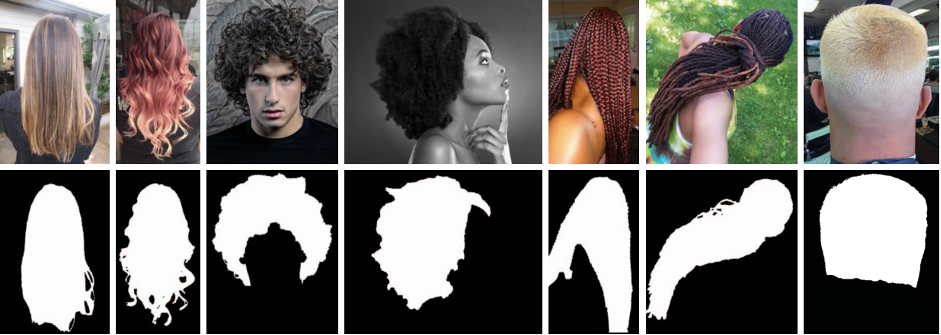
\includegraphics[width=0.9\textwidth]{chapter4/image/figaro.png}
    \caption{Examples of image and mask in Figaro1k dataset}
    \label{fig:figaro}
\end{figure}

Figaro1k consists of 1050 images, equally distributed in seven hairstyle classes. It is regarded as an annotated novel multi-class image database for hair analysis in the wild.

\paragraph{LFW}
LFW,  stands for "Labeled Faces in the Wild", is also an annotated face dataset in the wild dataset. It contains more than 2,000 images of faces collected from the web. Each face has been labeled with the name of the person pictured so that the dataset is also used as the benchmark for the face recognition problem.

\begin{figure} [H]
    \centering
    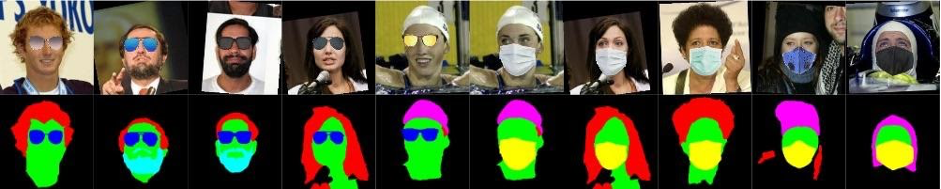
\includegraphics{chapter4/image/lfw.png}
    \caption{Examples of image and mask in LFW dataset}
    \label{fig:lfw}
\end{figure}

Each image is a JPG image with the size of 250x250. The dataset is already split into train, validation, and test set. They have respectively 1500 images, 500 images, and 900 images.